% !TeX root = ../solution.tex

\hypertarget{he22.28}{%
\chapter{[HE22.28] C0ns0n4nt Pl4n3t}\label{he22.28}}

\begin{marginfigure}
	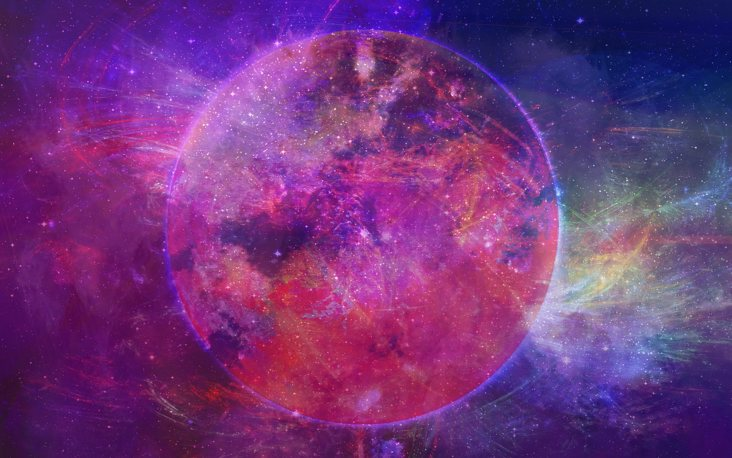
\includegraphics[width=49mm]{level7/challenge28.jpg}
\end{marginfigure}
\section{Intro}
\textbf{Apollo} wants his name printed on that fancy new site. He's constantly failing as vowels and some special characters are blocked when entered.

\noindent Can you help him?

\noindent \url{http://46.101.107.117:2205}

\noindent Note: The service is restarted every hour at x:00.
\section{Hint}
Submit \verb+"+ and see what happens.

\section{Solution}\label{hv22.28solution}

Using the hint, we find out that the server is running php.  Playing around with the hints at \href{https://github.com/swisskyrepo/PayloadsAllTheThings/tree/master/Command%20Injection#bypass-characters-filter-via-hex-encoding}{swissky}, we see that we can bypass the detection of vowels using hex escapes.  Submitting \verb+\x41p\x6fll\x6f+ (encoded for Apollo) greets us with the flag.

\noindent \verb+he2022{v0w3ls_4r3_f0r_n3rd5!}+





	









